\section{Immersed Bodies}
\label{sec_boddies}

One of the distinct features of {\psiboil} is it's ability to solve problems in
complex computational domains using an immersed boundary method~(IBM). For such cases, 
computational domain is divided into a {\em fluid} part, where all governing 
equations for heat transfer and fluid flow are solved, and the {\em solid} part, 
where no momentum equations are solved. However, in case of conjugate heat transfer
problems, heat transfer equations is solved in the solid part as well. 

In {\psiboil} solid parts of the computational domain are defined as
{\em immersed boundaries}, represented by the class {\tt Body}. These immersed
bodies (IB's) are defined by a computer aided design~(CAD) files in 
ASCII stereolitography~(STL) format. The creation of CAD files is performed by
a third party program. At PSI we use AC3D\footnote{\tt http://www.inivis.com/}, 
but any other CAD software package able to export ASCII STL file format could be used. 
This tutorial does not cover the usage of AC3D, nor any other CAD packages. It is
important, however, to mention the convention adopted in {\psiboil} concerning
IB's: {\em normals on the body surface point to the fluid part
of the domain}.

The usage of IB is illustrated in the following example. Consider a case of a domain
with dimensions: $4 \times 1 \times 1$ in $x$, $y$ and $z$ direction
respectively, with a step-like obstacle with dimension 
$0.5 \times 1.0 \times 0.5$ placed at the bottom wall (minimum $z$) 
of the domain. Immersed body is created in AC3D and stored in the file named {\tt step.stl}.
The dimensions of the IB are set to be slightly larger in CAD program
to avoid ambiguity when cutting cells. In effect, the actual dimensions of the IB are
$0.501 \times 1.001 \times 0.501$.
This file should be stored in the running directory. The program which uses the~STL
file to create a mesh for a domain with a step-like obstacle is ({\tt 05-06-main.cpp}): 
%
{\small \begin{verbatim}
      1 #include "Include/psi-boil.h"
      2
      3 const real LX = 4.0;
      4 const real LY = 1.0;
      5 const int  NX =  64;
      6 const int  NY =  16;
      7
      8 /******************************************************************************/
      9 main(int argc, char * argv[]) {
     10
     11   boil::timer.start();
     12
     13   /* plot in Tecplot format */
     14   boil::plot = new PlotTEC();
     15
     16   /* grids */
     17   Grid1D g_x( Range<real>(0,LX), NX, Periodic::no() );
     18   Grid1D g_y( Range<real>(0,LY), NY, Periodic::no() );
     19
     20   /* create immersed body */
     21   Body step("05-06-step.stl");
     22
     23   /* plot step before immersion */
     24   boil::plot->plot(step, "step-before");
     25
     26   /* create domain */
     27   Domain dom(g_x, g_y, g_y, &step);
     28
     29   /* plot step after immersion */
     30   boil::plot->plot(step, "step-after");
     31
     32   /* plot domain after immersion */
     33   boil::plot->plot(dom, "dom-after");
     34
     35   boil::timer.stop();
     36   boil::timer.report();
     37 }
\end{verbatim}}
%
Program lines from~1--18 should be clear at this point. {\tt Body} is created
in line 21. It is defined with the STL file name containing IB definition. As soon
as the {\tt Body} is created, it is plotted from line~24. This plotting is not
necessary, of course, but can be useful for checking. 

Problem domain is defined in line~27. The novelty in this constructor is the 
final argument, a reference to {\tt Body} (an IB). {\tt Domain}'s constructor will cut 
the computational cells with IB, but also change the IB itself. 
Line~30 plots the IB after cutting and line~33 the final computational domain.
If you compile and run this program, it will create the following output:
%
{\small \begin{verbatim}
# Plotting: step-before_p000.dat
Domain level 4 created !
Domain level 3 created !
Domain level 2 created !
Domain level 1 created !
# Plotting: sca_p000.dat
# Plotting: vec_p000.dat
# Plotting: step-after_p000.dat
# Plotting: dom-after_p000.dat
+==========================================
| Total execution time: 0.29 [s]
+------------------------------------------
| Time spent in plotting    : 0.24 [s]    (82.7586%)
| Time spent in bounding box: 0 [s]    (0%)
| Time spent in cell cutting: 0.02 [s]    (6.89655%)
| Time spent in flood fill  : 0.01 [s]    (3.44828%)
| Time spent elsewhere      : 0.02 [s]    (6.89655%)
+------------------------------------------
\end{verbatim}}
%
File containing IB before immersing (cutting) is called {\tt step-before\_p000.dat},
while the IB after immersing is stored in file {\tt step-after\_p000.dat}. They are
plotted in Figs.~\ref{fig_body_before} and~\ref{fig_body_after}, respectively. 

%--------%
%        %
%  Body  %
%        %
%--------%
\begin{figure}[ht!]
  \centering
  \setlength{\unitlength}{1mm}
  \begin{picture}(103,53)(0,0)
    \thickbox{103}{53}
    \put(0,-20){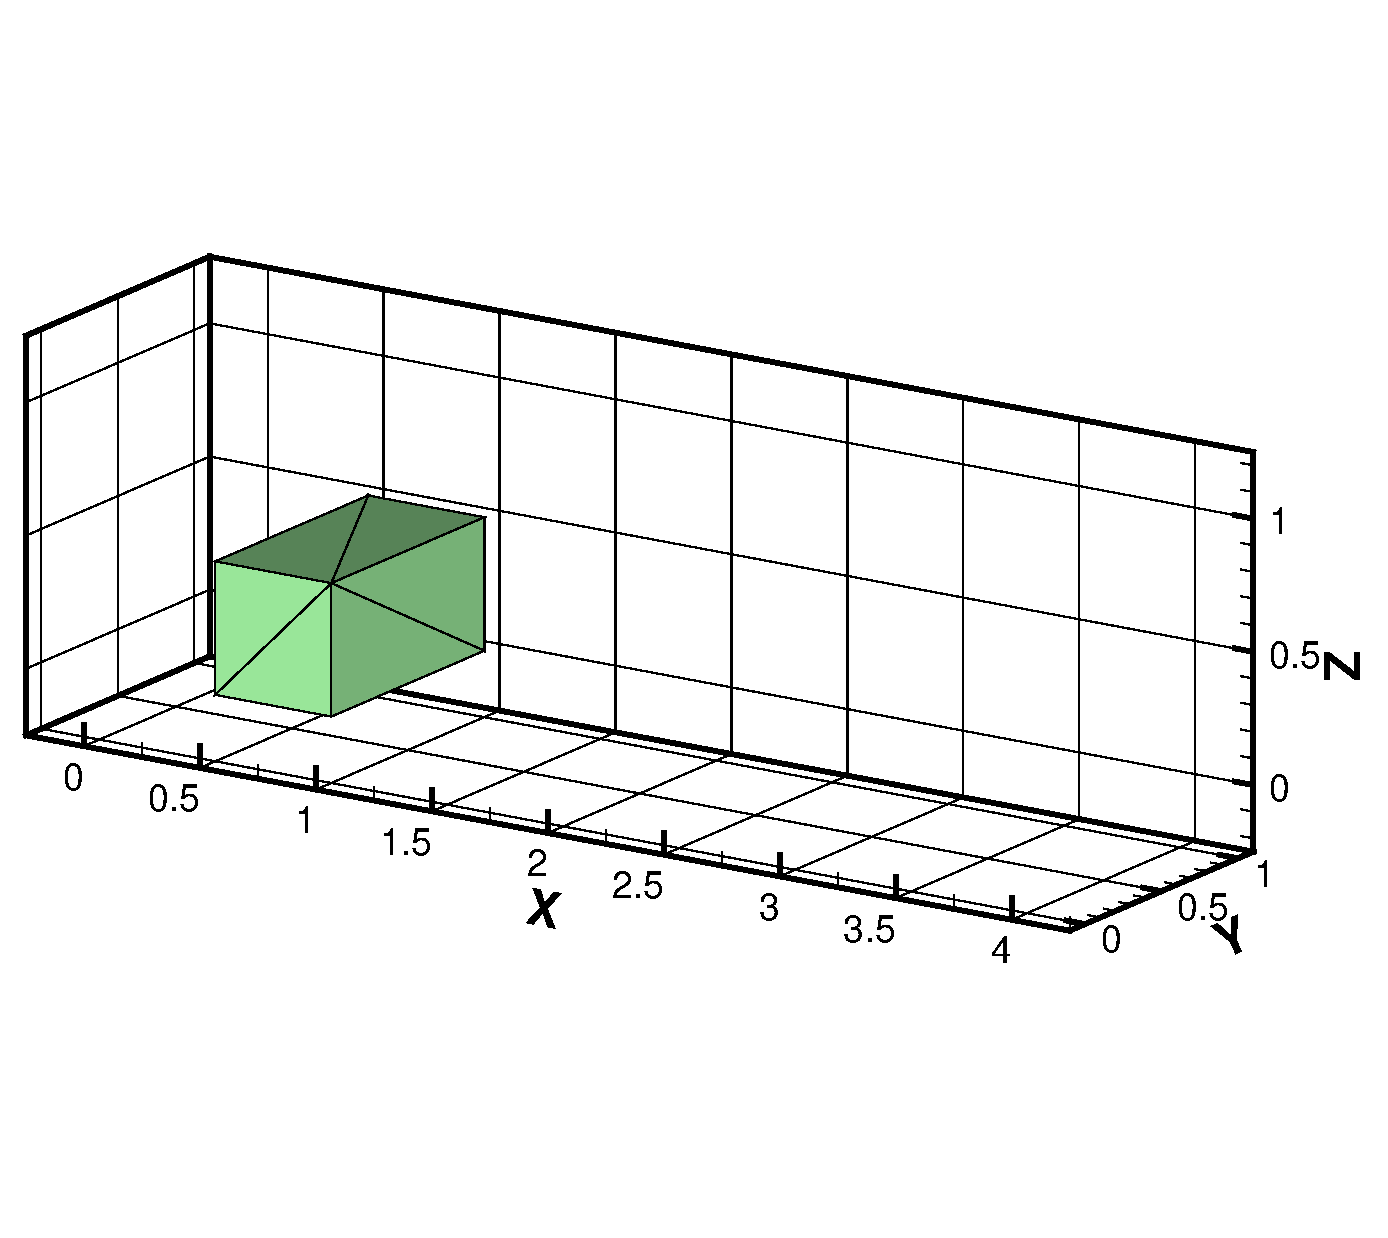
\includegraphics[scale=0.45]{Figures/05-06-body-before.eps}}
  \end{picture}
  \caption{IB plotted from line~24, {\em i.e.} before immersing it into
           computational domain. At this point it is the same as it was 
           defined in a CAD program.}
  \label{fig_body_before}
\end{figure}

In addition to the IB and domain files described above, {\psiboil} creates two
additional files: {\tt sca\_p000.dat} and {\tt vec\_p000.dat}. These files hold
scalar and vector respectively, representing ratio of the computational cell 
volume immersed in fluid. So, for cells inside the fluid part of the domain, 
it's value is~$1$, in the solid part it is~$0$, and for cells which are cut by 
immersed body, it's value is between~$0$ and~$1$. {\tt sca\_p000.dat} holds these 
values for scalar variables, while {\tt vec\_p000.dat} holds vector values. It is
a good practice to visualize these fields, just to visually check if IB is 
properly handled by {\psiboil}. Visualization of~{\tt sca\_p000.dat} is given
in Fig.~\ref{fig_scalar_obst_1}.

%--------%
%        %
%  Body  %
%        %
%--------%
\begin{figure}
  \centering
  \setlength{\unitlength}{1mm}
  \begin{picture}(103,53)(0,0)
    \thickbox{103}{53}
    \put(0,-20){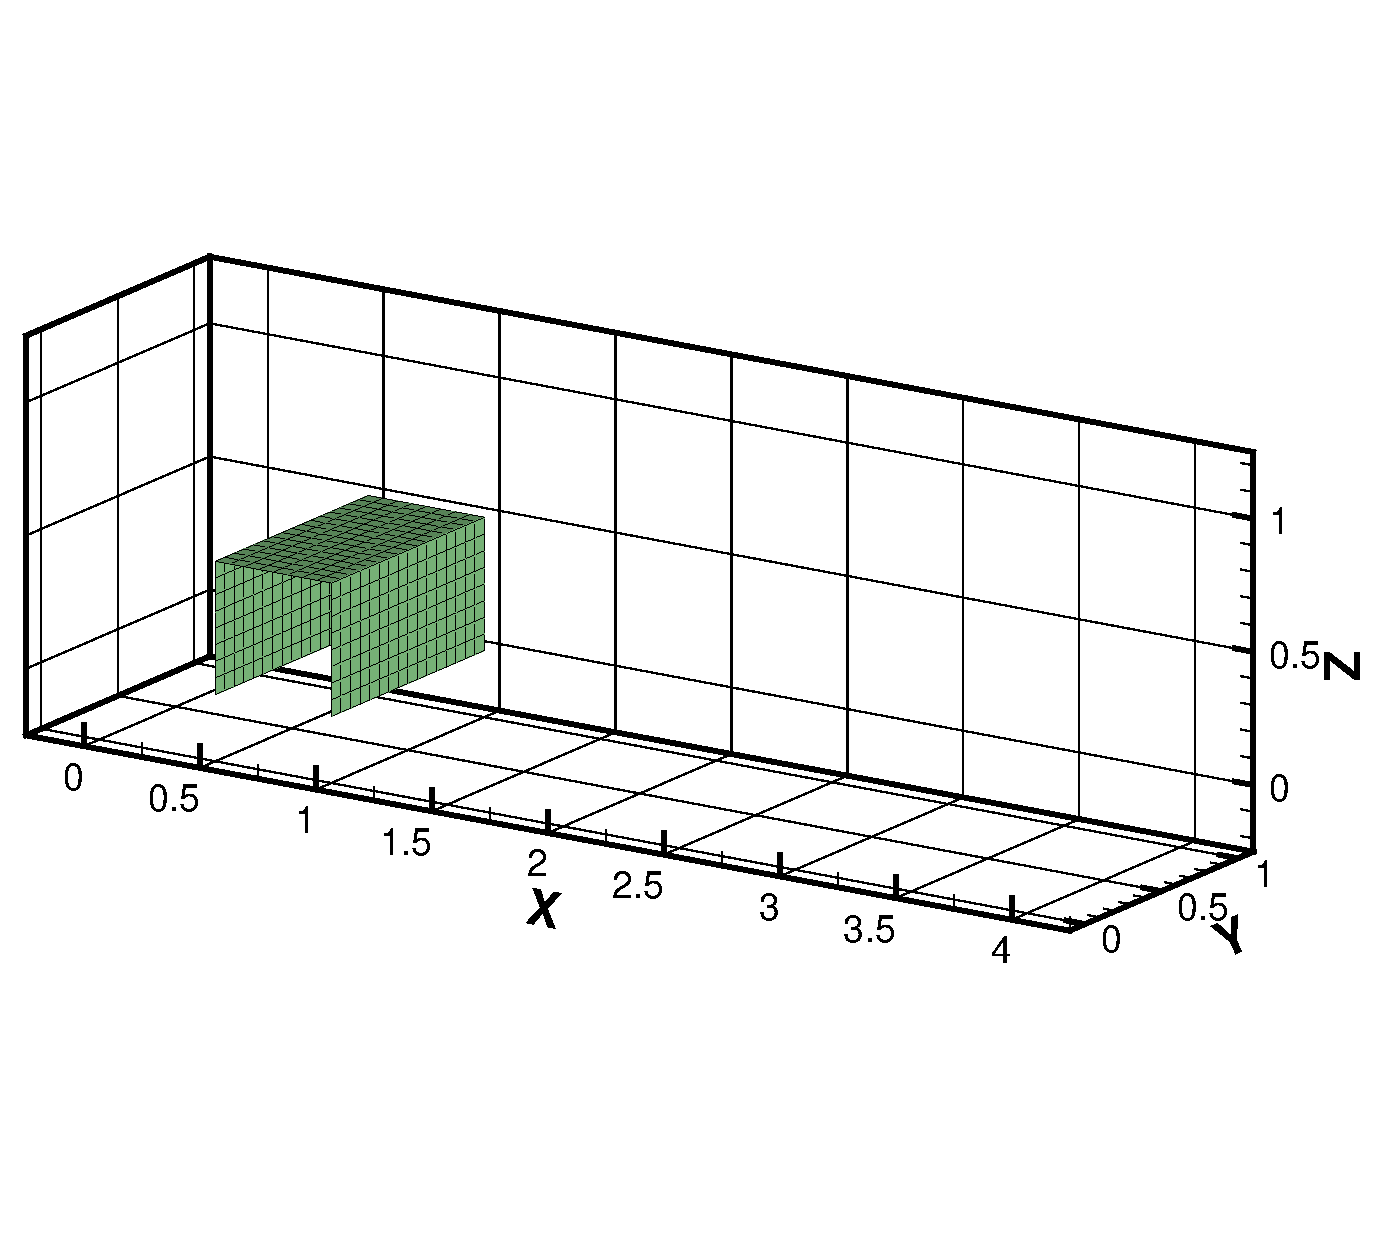
\includegraphics[scale=0.45]{Figures/05-07-body-after.eps}}
  \end{picture}
  \caption{IB plotted from line~30, {\em i.e.} after immersing it into
           computational domain. At this point, the topology of the IB  
           has changed; the original triangles are replaced by cell cuts.}
  \label{fig_body_after}
\end{figure}

%----------%
%          %
%  Domain  %
%          %
%----------%
\begin{figure}
  \centering
  \setlength{\unitlength}{1mm}
  \begin{picture}(103,53)(0,0)
    \thickbox{103}{53}
    \put(0,-20){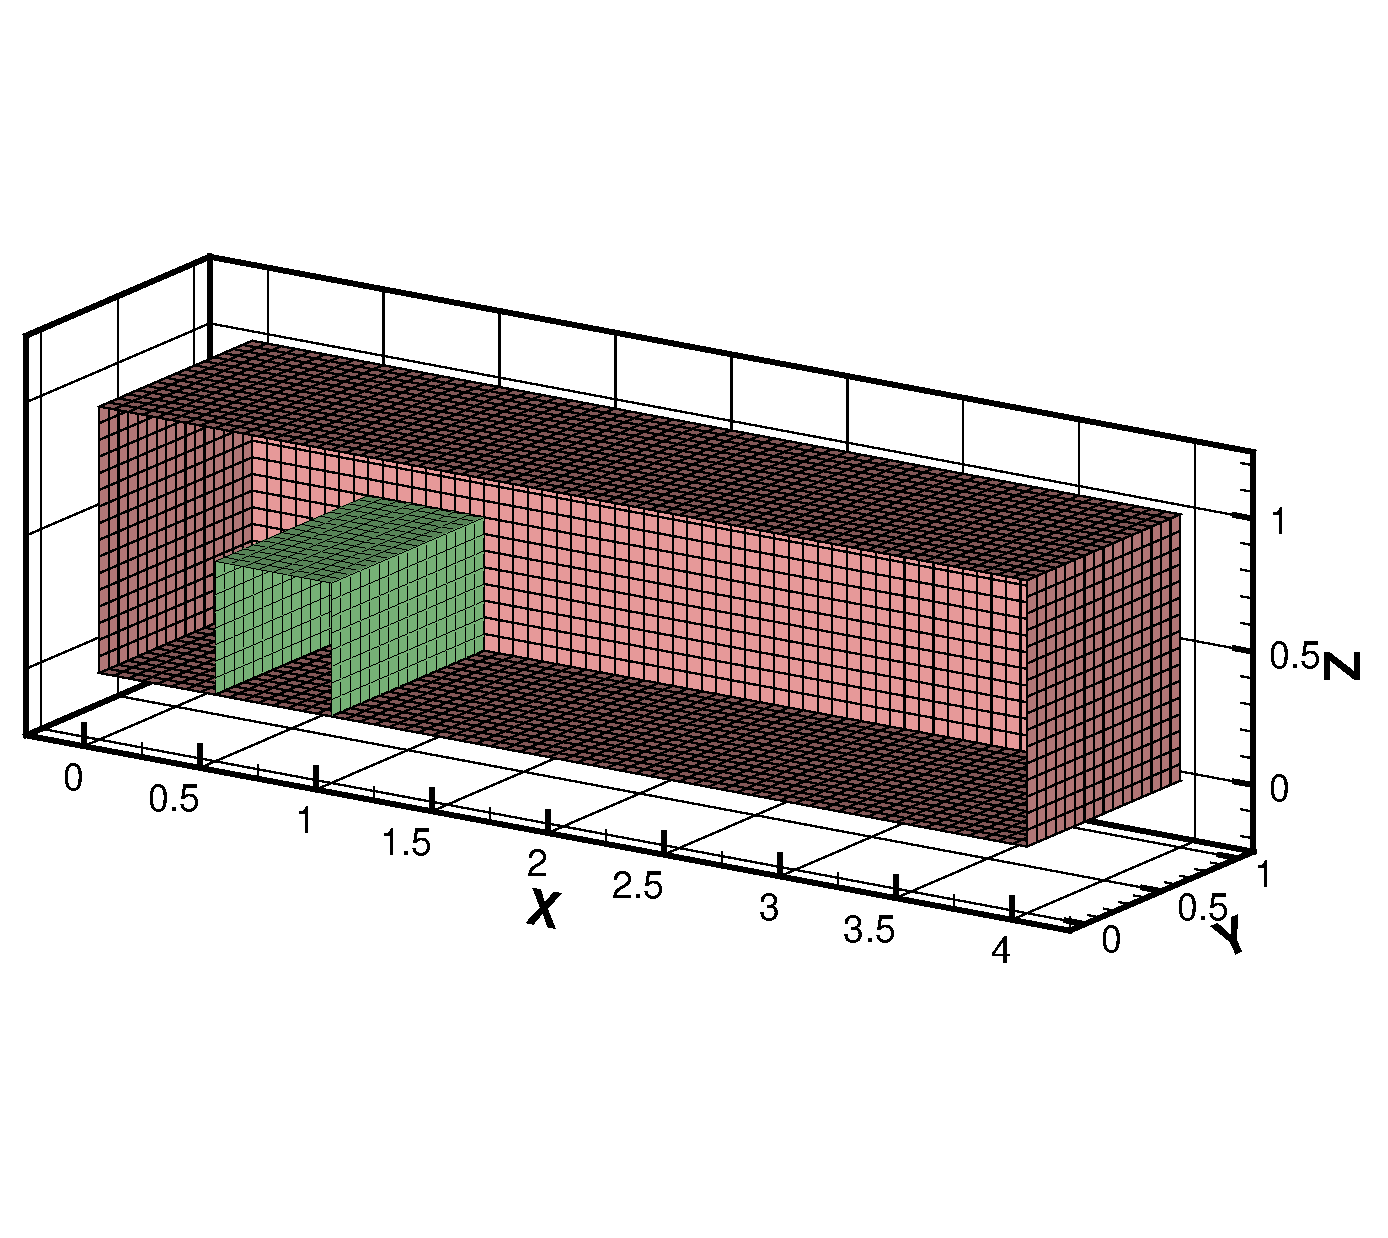
\includegraphics[scale=0.45]{Figures/05-08-domain.eps}}
  \end{picture}
  \caption{Computational domain with IB. Domain is colored in pink and obstacle 
           in green. The front face is removed from the figure for the sake of clarity.}
  \label{fig_domain_obst_1}
\end{figure}

%----------%
%          %
%  Scalar  %
%          %
%----------%
\begin{figure}
  \centering
  \setlength{\unitlength}{1mm}
  \begin{picture}(103,53)(0,0)
    \thickbox{103}{53}
    \put(0,-20){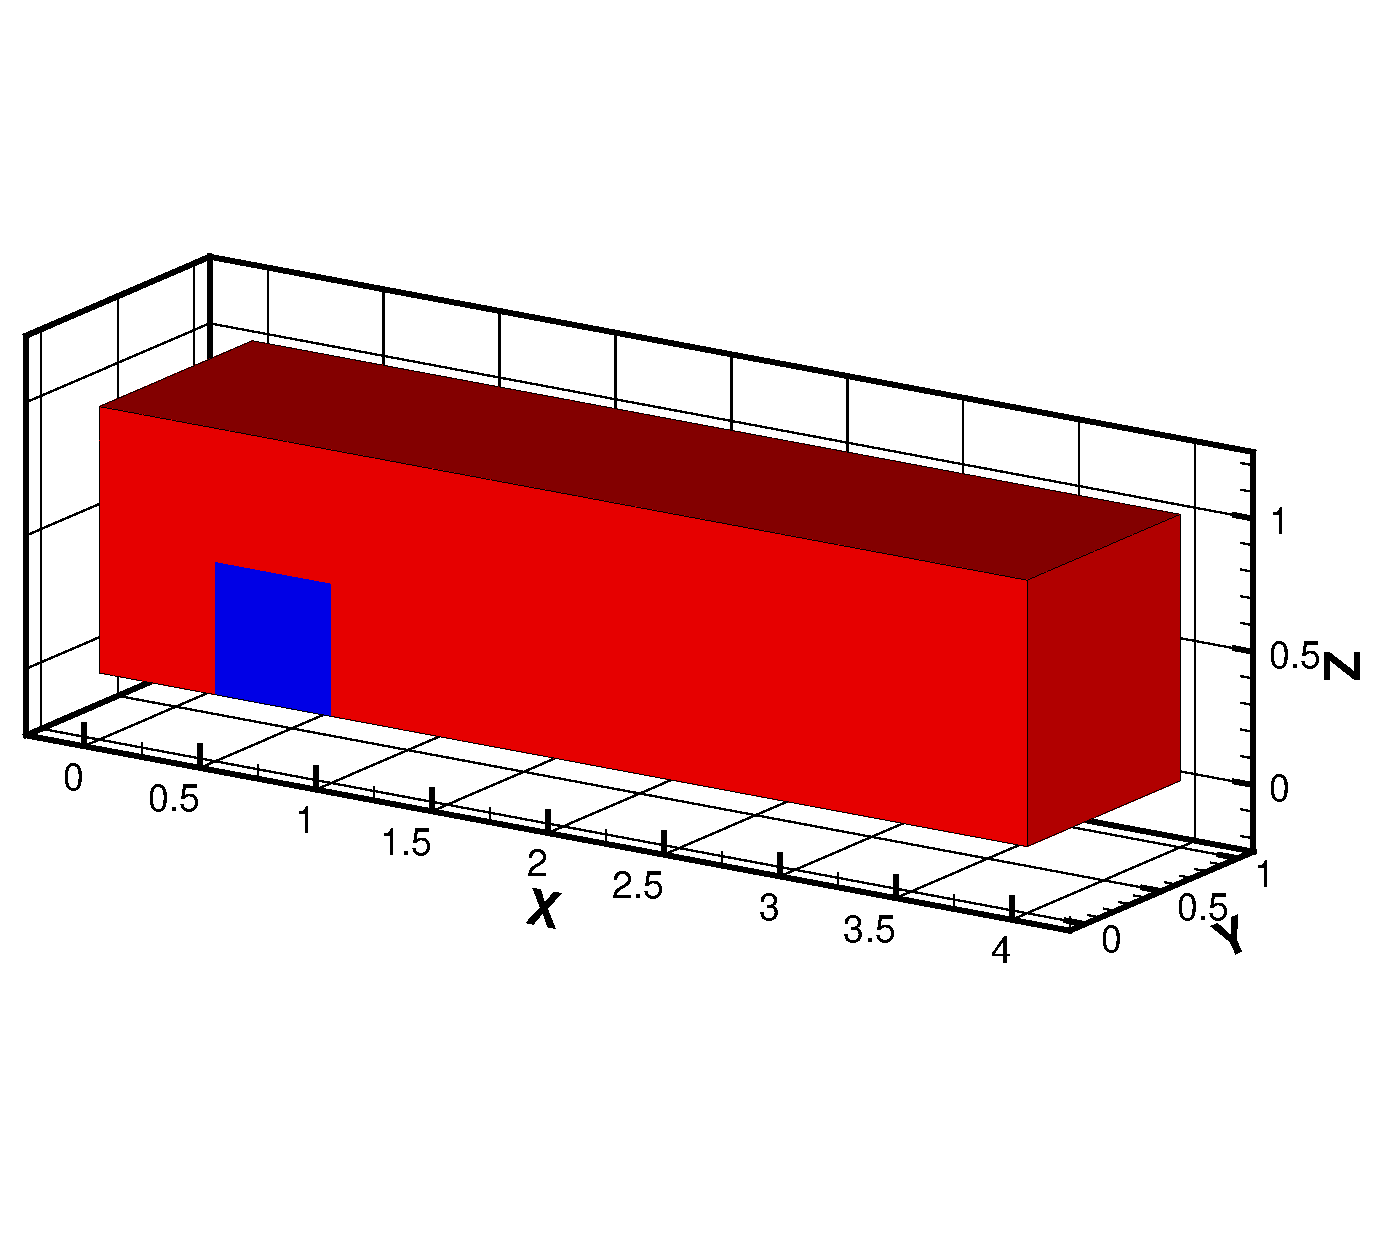
\includegraphics[scale=0.45]{Figures/05-09-sca.eps}}
  \end{picture}
  \caption{Scalar field representing volume fraction of the cell immersed in fluid.}
  \label{fig_scalar_obst_1}
\end{figure}

%---------------------------------------------------------------------nutshell-%
\vspace*{5mm} \fbox{ \begin{minipage}[c] {0.97\textwidth} %-----------nutshell-%
    {\sf Section \ref{sec_boddies} in a nutshell} \\  %-------------nutshell-%
    
      - To deal with problems in complex geometries, {\psiboil} divides computational 
      {\tt Domain} into {\em fluid} and {\em solid} part. \\

      - Solid part is represented with an object of type {\tt Body}, while fluid
      is everywhere else. \\

      - By convention, the CAD file representing the {\tt Body} has surface 
      normals oriented toward the fluid part of the computational domain. \\

      - {\tt Body} is an object created from a 3D CAD file as following:
      \begin{itemize}
        \item {\tt Body body(const std::string name);}  
      \end{itemize}
      where {\tt name} is the name of the CAD file in ASCII STL format. \\

      - {\tt Body} is inserted into a {\tt Domain}, using the constructor:
      \begin{itemize}
        \item {\tt Domain(Grid1D \&, Grid1D \&, Grid1D \&, Body *);}
      \end{itemize}
      {\tt Body} is sent as a pointer to {\tt Domain} because it changes 
      during the process of computational cell cutting.
   
  \end{minipage} } %--------------------------------------------------nutshell-%
%---------------------------------------------------------------------nutshell-%
